\documentclass[iop,numberedappendix,apj,]{emulateapj}

\usepackage{epsfig}
\usepackage{amsmath}
\usepackage{rotating}
\usepackage{natbib}
\usepackage{enumerate}
\usepackage{multirow}
\usepackage{array}
\usepackage{appendix}
\usepackage{comment}
\usepackage{color,xcolor}
\usepackage{url}
\usepackage{here}
\usepackage{hyperref}
\hypersetup{colorlinks,linkcolor={blue!50!black},citecolor={blue!50!black},urlcolor={blue!50!black}}
\allowdisplaybreaks[1]
\bibliographystyle{apj}
\renewcommand{\bibname}{References}

\def\plotonesc#1{\centering \leavevmode
\includegraphics[clip=, width=1.70\columnwidth]{#1}}
\def\plotoneh#1{\centering \leavevmode
\includegraphics[clip=, width=.95\columnwidth]{#1}}
\def\plotone#1{\centering \leavevmode
\includegraphics[clip=, width=.85\columnwidth]{#1}}
\def\plotoneShrinkSmall#1{\centering \leavevmode
\includegraphics[clip=, width=.49\columnwidth]{#1}}
\def\plotoneShrinkMed#1{\centering \leavevmode
\includegraphics[clip=, width=.55\columnwidth]{#1}}
\def\plotoneShrinkBig#1{\centering \leavevmode
\includegraphics[clip=, width=.65\columnwidth]{#1}}
\def\plottwo#1#2{\centering \leavevmode
\includegraphics[width=.45\columnwidth]{#1} \hfil
\includegraphics[width=.45\columnwidth]{#2}}
\def\plottwob#1#2{\centering \leavevmode
\includegraphics[width=.49\columnwidth]{#1} \hfil
\includegraphics[width=.49\columnwidth]{#2}}
\def\plottwor#1#2{\centering \leavevmode
\includegraphics[width=.55\columnwidth,angle=90]{#1} \hfil
\includegraphics[width=.55\columnwidth,angle=90]{#2}}
\def\plotthree#1#2#3{\centering \leavevmode
\includegraphics[width=.3\columnwidth]{#1} \hfil
\includegraphics[width=.3\columnwidth]{#2} \hfil
\includegraphics[width=.3\columnwidth]{#3}}

\def\gsim{\;\rlap{\lower 2.5pt
 \hbox{$\sim$}}\raise 1.5pt\hbox{$>$}\;}
\def\lsim{\;\rlap{\lower 2.5pt
   \hbox{$\sim$}}\raise 1.5pt\hbox{$<$}\;}
%\def\fast{\;$f^{\ast }$\;}
\def\fast{\tilde f}

% set formatting properties
\setlength{\textwidth}{6.5in}
\setlength{\textheight}{8.8in}
\setlength{\hoffset}{0.0in}
\setlength{\voffset}{-0.4in}
\parindent 0.2in
\parskip 0.1in

\def\memoYF#1{\color{red}[NOTE: {\bf #1}]\color{black}}


%%% http://www.oceanwave.jp/index.php?float%B4%C4%B6%AD(figure%2Ftable)%A4%CE%BD%D0%CE%CF%B0%CC%C3%D6%A4%F2%A5%B3%A5%F3%A5%C8%A5%ED%A1%BC%A5%EB

%%%%%%%%%%%%%%%%%%%%%%%%%%%%%%%%%%%%%%%%%%%%%%%%%
% THE DOCUMENT BEGINS HERE                      %
%%%%%%%%%%%%%%%%%%%%%%%%%%%%%%%%%%%%%%%%%%%%%%%%%

%\slugcomment{Submitted to ApJ, XX September 2015}

\begin{document}

\title{(tentative) Rotational Spectral Unmixing of Exoplanets}


\author{
%
Yuka Fujii\altaffilmark{1,2} 
%
Jacob Lustig-Yaeger\altaffilmark{3} 
%
Nicolas Cowan\altaffilmark{4} 
%
}

\affil{$^1$NASA Goddard Institute for Space Studies, 
  New York, NY 10025, USA}
      
\affil{$^2$Earth-Life Science Institute, Tokyo Institute of Technology, 
  Tokyo, 152-8550, JAPAN}
  
  
\affil{$^3$University of Washington, 
  }

\affil{$^4$McGill University, 
  }


\vspace{0.5\baselineskip}

\email{
yuka.fujii.ebihara@gmail.com
}

\begin{abstract}

\end{abstract}

\keywords{planets and satellites: Jupiter --- Sun: evolution ---
  planetary systems --- stars: evolution ---
  stars: AGB and post-AGB --- radio continuum: planetary systems}
  
%]%%% End front material



%%%%%%%%%%%%%%%%%%%%%%%%%%%%%%%%%%%%%%%%%%%%%%%%%%%%%%%%%%%%%%%%%%%
\section{Introduction}
\label{sec:intro}
%%%%%%%%%%%%%%%%%%%%%%%%%%%%%%%%%%%%%%%%%%%%%%%%%%%%%%%%%%%%%%%%%%%

Future direct imaging observations of terrestrial exoplanets is expected to play a vital role in characterizing Earth analogs in habitable zones and beyond. 
A substantial number of work have seeked detectable features in disk-integrated spectra of the Earth and other planets, as they are observed from an astronomical distance. 
It has been pointed out that not only some of atmospheric molecules are identifiable through spectral absorption features \citep[e.g.,][]{DesMarais2002} but also surface reflectance spectra affect the continuum of the spectra, which could be measured through low-resolution spectra, or multi-band photometry (color) \citep[e.g.,][]{Ford2001}. 

However, interpretation of disk-integrated colors is not trivial. 
This is particularly true for Earth-like planets that harbor diverse atmospheric and surface characteristics including liquid water, partial cloud cover, continents, and possible biological surfaces, e.g. vegetation. 
Disentangling specific features from the mixed disk-integrated colors can be very challenging. 

A key here is to use time variation of the spectra; because the surface area that contributes to the scattered light changes due to the planetary spin rotation and the orbital revolution, the time variability can in principle be translated to the heterogeneity of the surface environment.  
\citet{Cowan2009, Cowan2011} performed Principal Component Analysis (PCA) on the observed multi-band photometry of the Earth, and found that number of surface types can be inferred from the number of dominant principle components; (\# of surface types) $\ge $ (\# of principal componentes) $+ 1$. %) and that the variation pattern is indicative of the surface properties. 
\citet{Fujii2010, Fujii2011} decomposed multi-band photometric data of the Earth as a linear inverse problem, assuming the template reflectance spectra of the known major surface types, and they found that the relative abundance and the longitudinal variation of these surface types are reasonably recovered. 
Moreover, by coupling the time variation due to spin rotation and that due to orbital revolution, 2-dimensional information of the surface may be retrieved with sufficient quality of data \citep{Kawahara2010, Kawahara2011, Fujii2012}. 

\citet{Cowan2013} took another approach to the same inverse problem. 
Their strategy is to try to estimate the physically meaningful reflectance spectra and their distribution across the globe simultaneously, by making all of them fitting parameters and letting them fit the data. 
The result appeared successful to the extent that the obtained reflectance spectra roughly match the typical spectra of clouds, ocean, and continents. 
However, the longitudinal map of these components do not match the reality sufficiently well. 

We were motivated by this unsatisfactory result and decided to revisit their analysis with some updates. 
Specifically, the updates include:
\begin{itemize}
\item Revisiting the formulation and point out the inherit degeneracy. 
\item Introducing regularization terms
\item Influence of the unknown radius
\end{itemize}

The organization of this paper is as follows. 
Section \ref{s:frame} revisits the problem, ....

\newpage

%%%%%%%%%%%%%%%%%%%%%%%%%%%%%%%%%%%%%%%%%%%%%%%%%%%%%%%%%%%%%%%%%%%
\section{Framing the problem}
\label{s:frame}
%%%%%%%%%%%%%%%%%%%%%%%%%%%%%%%%%%%%%%%%%%%%%%%%%%%%%%%%%%%%%%%%%%%


%%%%%%%%%%%%%%%%%%%%%%%%%%%%%%%%%%%%%%%%%%%%%%%%%%%%%%%%%%%%%%
\subsection{Algebraic Formulation}
\label{ss:model}
%%%%%%%%%%%%%%%%%%%%%%%%%%%%%%%%%%%%%%%%%%%%%%%%%%%%%%%%%%%%%%

Assuming that the planetary surface is Lambertian scatterer everywhere, with a certain number $K$ of spectrally distinct surface types, 
the disk-integrated scattered light can be written as a weighted summation of the reflectance spectra of different surface types. 

For the moment, let us suppose that the planetary radius and the observational geometry (latitude/longitude of the sub-stellar/sub-observer points, and the distance between the star and the planet) are fully known. (This will be relaxed in \S\ref{s:discussion}.) 
In this case, we can straightforwardly translate the observed planetary intensity to albedo (or reflectivity) using the stellar flux. 
A useful normalization for albedo in exoplanet observations is {\it apparent albedo}, which is the planetary intensity normalized by that of a loss-less Lambert sphere with the same radius and at the same phase \citep{Qiu2003, Seager2010}; in this paper we will consistently use apparent albedo for our study unless otherwise noted. 

The observed apparent albedo, $d_{ij}$ (``$d$'' for data), can be written as \citep[see][]{Fujii2010}: 
%%%
\begin{eqnarray}
d_{i} (\lambda_j) &=& \displaystyle \frac{ \int_{{\rm IV}_i} s_{\vec \Omega }(\lambda_j) \cdot \cos \theta_0 ({\vec \Omega}) \cdot \cos \theta_1 ({\vec \Omega}) \cdot d\vec \Omega }{ \int_{{\rm IV}_i}  \cos \theta_0 ({\vec \Omega}) \cdot \cos \theta_1 ({\vec \Omega}) \cdot d\vec \Omega } \\
&=& \sum _{k} s_k (\lambda_j) \; \displaystyle \frac{ \int_{{\rm IV}_{i}} f_k (\vec \Omega ) \cos \theta_0 ({\vec \Omega}) \cdot \cos \theta_1 ({\vec \Omega}) \cdot d\vec \Omega }{ \int_{{\rm IV}_i}  \cos \theta_0 ({\vec \Omega}) \cdot \cos \theta_1 ({\vec \Omega}) \cdot d\vec \Omega } \\
&\equiv & \sum _{i,k} \fast_{ik} \, s_{kj} \label{eq:d_f_ast_s}
\end{eqnarray}
%%%
where $i$, $j$, and $k$ are indices for the observation epochs, bands, and the surface types, respectively, ${\rm IV }_i$ denotes the illuminated and visible area over the planetary surface at $i$-th observation, and $f (\vec \Omega )$ is the area fraction of $k$-th surface type in $d\vec \Omega$. 
In the last expression, $\fast_{lk}$ represents the apparent covering fraction of the $k$-th surface type at $i$-th observational epoch, and 
$s_{kj}$ is the reflectance spectra of $k$-th surface type at $j$-th band. 
The maximum number of $i$, $j$ and $k$ will be denoted by $I$, $J$, and $K$, below, as summarized in Table \ref{tab:index}. 

By definition, the area fraction $\fast $ and reflectance spectra $s$ are subject to the following conditions:
%%%
\begin{eqnarray}
\begin{cases}
\;\; 0 < s_{kj} < 1 \;\;\; & \mbox{for any $k$, $j$} \\
\;\; 0 < \fast_{lk} < 1 \;\;\; & \mbox{for any $l$, $k$} \label{eq:cond_f_ast}\\
\;\; \sum_k \fast_{lk} = 1 & \mbox{for any $l$} 
\end{cases}
\end{eqnarray}
%%%


%%%%%%%%%%%%%%%%%%%%%%%%%%%%%%%%%%%
\begin{table}[tbh]
\caption{Indexes}
\begin{center}
\begin{tabular}{ccc} \hline \hline
Name & Symbol & Maximum \\ \hline
Observation Time & $i$ & I \\
Band & $j$ & J  \\
Surface Type & $k$ & K  \\
Longitudinal Slice  & $l$ & L \\ \hline
\end{tabular}
\end{center}
\label{tab:index}
\end{table}%
%%%%%%%%%%%%%%%%%%%%%%%%%%%%%%%%%%%

The time variability of the apparent covering fraction $\fast $ due to spin rotation is related to the surface inhomogeneity along the equator. Approximately, $\fast _{ik}$ may be written as the weighted summation of the area fraction of $k$-th surface type in each of (the finite number $L$ of) longitudinal slices, i.e.,
%%%
\begin{eqnarray}
\fast _{ik} &=& \frac{ \int_{{\rm IV}_{i}} f_k (\vec \Omega ) \cos \theta_0 ({\vec \Omega}) \cdot \cos \theta_1 ({\vec \Omega}) \cdot d\vec \Omega }{ \int_{{\rm IV}_i}  \cos \theta_0 ({\vec \Omega}) \cdot \cos \theta_1 ({\vec \Omega}) \cdot d\vec \Omega }  \\
&=& \sum_l \frac{ \int_{{\rm IV}_{il}}  f_k (\vec \Omega ) W (\vec \Omega  ) \cdot d\vec \Omega }{ \int_{{\rm IV}}  W (\vec \Omega ) \cdot d\vec \Omega } \\
&\sim & \sum_l f_{lk} \frac{ \int_{{\rm IV}_{il}} W (\vec \Omega ) \cdot d\vec \Omega }{ \int_{{\rm IV}}  W (\vec \Omega ) \cdot d\vec \Omega } \label{eq:discretize}\\
&\equiv & \sum_l  W_{il} f_{lk} \label{eq:Wf}
\end{eqnarray}
%%%
where $l$ is the index for longitudinal slices, $f_{lk}$ is the area fraction of the $k$-th surface type in the $l$-th longitudinal slice. 
Strictly speaking, the approximation is valid only when $f_k(\vec \Omega)$ does not change or changes little across the $l$-th slice for all $k$ and $l$. 
In the last equation, $W_{il}$ is the weight function for $i$-th epoch and $l$-th longitudinal slice which depends only on the observational geometry. 
As a result,
%%%
\begin{equation}
d_{ij} = R_p^2 \sum _{l,k} W_{il} \, f_{lk} \, s_{kj} \label{eq:d_f_s}
\end{equation}
%%%
with the following condition similar to equation (\ref{eq:cond_f_ast}):
%%%
\begin{eqnarray}
\begin{cases}
\;\; 0 < s_{kj} < 1 \;\;\; & \mbox{for any $k$, $j$} \\
\;\; 0 < f_{lk} < 1 \;\;\; & \mbox{for any $l$, $k$} \label{eq:cond_f} \\
\;\; \sum_k f_{lk} = 1 & \mbox{for any $l$} 
\end{cases}
\label{eq:constraints}
\end{eqnarray}
%%%
Now, the relevant problem is, given $d$, estimate $\{f, s\}$ subject to the constraints of equation (\ref{eq:constraints})---this is where \citet{Cowan2013} stood. 


\citet{Cowan2013} suggested the specific procedure to find the solution for $\{f, s\}$. 
Namely, 
(1) perform PCA on the data to reduce the dimensionality as needed, 
(2) perform simplex shrink-wrapping analysis to find the first guess for $s$, 
and 
(3) find the maximum posterior values for $\{f, s\}$ using MCMC algorithm  and setting the first guess for $s$ as the initial condition. 
(In the last step, the initial value for $f$ is fixed at 1/(\# of surface types).)

\newpage

%%%%%%%%%%%%%%%%%%%%%%%%%%%%%%%%%%%%%%%%%%%%%%%%%%%%%%%%%%%%%%
\subsection{Fit data with $\fast $ or with $f$ ?}
\label{ss:degeneracy}
%%%%%%%%%%%%%%%%%%%%%%%%%%%%%%%%%%%%%%%%%%%%%%%%%%%%%%%%%%%%%%

\memoYF{I am not 100\% sure if the following statement is right. Need to check. The argument below probably makes sense for the noiseless case. What if the data are noisy?}
 
We argue that estimating $\{ f, s \}$ is no superior to estimating $\{ \fast, s \}$. 
%
One reason comes from the approximation adopted in equation (\ref{eq:discretize}) is valid only when $f_k (\vec \Omega)$ does not change significantly in the $l$-th slice. 
Otherwise, fitting data with $f$ by equation (\ref{eq:Wf}) produces some errors by design. 

%Suppose the above approximation is justified. 
In essence, $f^{\ast }_{ik}$ and $f_{lk}$ contains the same information, where they are related through a fixed $W_{il}$ (eq. \ref{eq:Wf}). 
%
If $L=I$, in general there is a one-to-one relationship between $\fast_{ik}$ and $f_{lk}$ through $W_{il}$ as far as ${\rm rank}(W)=L(=I)$. 
In this case, clearly, equations (\ref{eq:cond_f_ast}) and (\ref{eq:cond_f}) are equivalent, given $W_{il}>0$ (for any $i$ and $j$) and $\sum _l W_{il} = 1$. 
%
If $L<I$, the matrix $W$ works as a low-pass filter \citep{Cowan2013}. 
In this case, the inverse problem described by equation (\ref{eq:Wf}), $\fast=Wf$, is an overdetermined system, and one must to find the solution for $f$ by some means (e.g. the least squares method), and the resultant $f$ may not automatically satisfy the condition listed by equation (\ref{eq:cond_f}). 

However, this is because of the design of the problem and the assumed lowered resolution. 

Therefore, although either $\{ \fast, s \}$ or $\{ f, s \}$ could be fitting parameters to the data, the estimation for $s$ should not be affected by this conversion in fitting parameters. 
In that sense, $\{ f, s \}$ is not likely to return a better solution than $\{ \fast, s \}$ does. 
Rather, it could return less reasonable results because of the approximation adopted in equation (\ref{eq:discretize}). 

\newpage

%%%%%%%%%%%%%%%%%%%%%%%%%%%%%%%%%%%%%%%%%%%%%%%%%%%%%%%%%%%%%%
\subsection{Degeneracy}
\label{ss:degeneracy}
%%%%%%%%%%%%%%%%%%%%%%%%%%%%%%%%%%%%%%%%%%%%%%%%%%%%%%%%%%%%%%

\memoYF{The degeneracy in solving $\{ \fast ,\,s\} $ is already indicated in \citet{Cowan2013}, but might be worth clarifying here again. }


One could try to find the solutions for $\{ \fast, s \}$ given $d$ using equation (\ref{eq:d_f_ast_s}), or the solutions for  $\{ f, s \}$ using equation (\ref{eq:d_f_s}), but we must keep in mind that 
these two formulations both embrace intrinsic degeneracies in the solutions if there is no other information about $\fast$ (or $f$) and $s$. 

%%%
%\begin{equation}
%d_{ij} = \sum _{i,k} f^{\ast }_{ik} \, s_{kj} \tag{\ref{eq:d_f_ast_s}}
%\end{equation}
%%%
%When one tries to find solutions for both $\fast$ and $s$ given $d$, the results are strongly degenerate if there are not other information about $\fast$ and $s$. 

Without any constraints on $\fast$ (or $f$) and $s$, it is trivial to notice the degeneracy in the solutions. 
Using an arbitrary regular matrix $X$ with rank $K$, a particular set of solution $\{ \fast ,\,s\}$ implies another set of solution $\{ \fast X^{-1},\,Xs\}$. 

Now that they are subject to the constraints (equation (\ref{eq:cond_f_ast}) or (\ref{eq:cond_f})), the range of the acceptable solution is limited. Nevertheless, the constraints cannot be sufficient to narrow them to a unique set of solution. 
%
To see this, %let us consider equation (\ref{eq:d_f_ast_s}) for the moment.
imagine a $J$-dimensional space.
Suppose there are $K$ number of vertices in that space, $\vec x_1,\,\vec x_2,\,...,\,\vec x_K$, and that all of the coordinate of $\vec x_k$ in this $J$-dimensional space is between 0 and 1. 
Mathematically, any points (say, $\vec y_1$, $\vec y_2$, ..., $\vec y_I$) that are {\it enclosed} in the hyperplane defined by these vertices may be represented by $\vec y_i=\sum _k^K p_{ik} \vec x_k $ where $\sum _k^K p_{ik} = 1$ for any $i$. 
%In the matrix form, $Y_{ij} = P_{ik} X_{kj}$. 
This is essentially same as the situation described by equation (\ref{eq:d_f_ast_s}). 

In other words, any set of vertices in $J$-dimensional space that can enclose all of the observed data, $\vec d_i$ can be the solutions for equation (\ref{eq:d_f_ast_s}), as long as all of the element in $x_{kj}$ satisfy $0<x_{kj}<1$. 
The condition $0<x_{kj}<1$ generally constrains the outer boundary of the possible locations for the vertices. 
Therefore, the ``answer'' vertices allowed by the observations are somewhere outside the polygon that tightly encloses the observed data and inside the outer boundary defined by the condition $0<x_{kj}<1$ (see \S\ref{ss:shrinkwrap} below). 

Note that in an exceptional case where the apparent covering fractions of all of the surface type come close to unity to different epochs, the allowed region for the vertices would be narrow, i.e., better estimation can be expected. 


\newpage

%%%%%%%%%%%%%%%%%%%%%%%%%%%%%%%%%%%%%%%%%%%%%%%%%%%%%%%%%%%%%%
\subsection{Bayesian Formulation ?}
\label{ss:regularization}
%%%%%%%%%%%%%%%%%%%%%%%%%%%%%%%%%%%%%%%%%%%%%%%%%%%%%%%%%%%%%%

Assuming the observational noise is distributed as Gaussian, 
%%%
\begin{eqnarray}
&&Posterior 
\\ &&= \prod\limits_{i,j}\left[  \frac{1}{\sqrt{2\pi }\sigma_{ij}} \exp \left\{ - \frac{(d_{ij} - \sum _{lk} W_{il} f_{lk} s_{kj})^2}{2 \sigma _{ij}^2} \right\} \right] \notag \\
&& \;\;\;\;\;\;\;\;\;\; \times \; \mathcal{P} (\{f_{lk}\}) \cdot \mathcal{P}(\{s_{kj}\}) 
\end{eqnarray}
%%%
where $\mathcal{P} (X) $ is a prior for $X$. 

In order to take account of constraints (equation (\ref{eq:constraints})), we adopt the following transformation of variables: 
%%%
\begin{eqnarray}
\begin{cases}
t_{kj} = \displaystyle \ln \left[ \frac{ s_{kj} }{1 - s_{kj} } \right]  \;\;\; & \mbox{for any $k$, $j$} \\
g_{lk} = \displaystyle \ln \left[ \frac{ f_{lk} }{1 - \sum _{m=0}^{k} f_{lm} } \right] \;\;\; & \mbox{for $k=1, ..., K-1$} %, any $j$} 
\end{cases}
\end{eqnarray}
%%%
Note that there is a 1-to-1 correspondence between $t$ and $s$ or $g$ and $f$ where $s$. 

\newpage

%%%%%%%%%%%%%%%%%%%%%%%%%%%%%%%%%%%%%%%%%%%%%%%%%%%%%%%%%%%%%%
\subsection{Prior: Gaussian Processes}
\label{ss:gp}
%%%%%%%%%%%%%%%%%%%%%%%%%%%%%%%%%%%%%%%%%%%%%%%%%%%%%%%%%%%%%%

\memoYF{This is just a quick draft and will need to be updated significantly.}

As seen in Section \ref{ss:degeneracy}, the solution is highly degenerate, and in general we cannot reduce to a unique solution. 
Therefore, we may want to give a prior in estimating the area fractions. 
What kind of assumptions can we make?

In general, the large time/longitude variations in apparent area fractions corresponds to spectrally similar surface types, because such solution correspond to the proximity of the inner boundary in the $J$-dimensional space discussed above. 
On the contrary, spectrally well-separated surface types correspond to small time/longitude variations in the apparent area fractions. 
In the real world, we might expect that the latter is more likely, i.e., covering area fraction of any surface type would not change significantly along the longitude (or in time). 
This would be a reasonable assumption for the estimation of $\{s, \fast \}$, since the illuminated and visible area is usually broad and tend to change the averaged area fraction of each surface type only gently. 
Although there is no physical proof for this assumption...

The assumption of the smoothness of the time variation of covering area fraction may be imposed using the concept of Gaussian Process \citep{Rasmussen2005}. 
We assume that the variation of the covering fraction follows Gaussian Process, which means the any finite number of the covering fractions have a joint Gaussian distribution. 
Such assumption can be represented by the prior of 
%%%
\begin{equation}
\mathcal{P}_{\fast} = \frac{1}{\sqrt{ 2 \pi }^{L(K-1)} \sqrt{| \tilde \Sigma |} } \exp( - \fast^{T} \tilde \Sigma ^{-1} \fast ) 
\end{equation}
%%%
or
%%%
\begin{equation}
\mathcal{P}_f = \frac{1}{\sqrt{ 2 \pi }^{L(K-1)} \sqrt{| \Sigma  |}} \exp( - f^{T} \Sigma ^{-1} f ) 
\end{equation}
%%%
where $\Sigma $ is the kernel representing the property of the gaussian processes assumed for $f$.
In this paper, we assume squared exponential covariance function, i.e., 
%%%
\begin{equation}
\tilde \Sigma _{ii'} = \lambda \exp \left( - \frac{|t_i- t_i'|^2}{2 (\Delta t_0) ^2} \right)
\end{equation}
%%%
where $t_i$ is the time of $i$-th observation and $(\Delta t_0)$ is characteristic time scale over which $\fast $ is supposedly correlated, or 
%%%
\begin{equation}
\Sigma _{ll'} = \lambda \exp \left( - \frac{|\phi_l- \phi_{l'}|^2}{2 \phi_0^2} \right)
\end{equation}
%%%
where $\phi_l$ is the longitude of $l$-th slice, and $\phi_0$ is the characteristic longitudes over which $f$ is correlated.  


\newpage

%%%%%%%%%%%%%%%%%%%%%%%%%%%%%%%%%%%%%%%%%%%%%%%%%%%%%%%%%%%%%%%%%%%
\section{Test with idealized mock data}
\label{s:mockdata}
%%%%%%%%%%%%%%%%%%%%%%%%%%%%%%%%%%%%%%%%%%%%%%%%%%%%%%%%%%%%%%%%%%%



%%%%%%%%%%%%%%%%%%%%%%%%%%%%%%%%%%%%%%%%%%%%%%%%%%%%%%%%%%%%%%
\subsection{Creating Mock Data}
\label{ss:createmockdata}
%%%%%%%%%%%%%%%%%%%%%%%%%%%%%%%%%%%%%%%%%%%%%%%%%%%%%%%%%%%%%%

%%%%%%%%%%%%%%%%%%%%%%%%%%%%%%%%%%%
\begin{figure*}[bth!]
    \begin{minipage}{0.5\hsize}
    \begin{center}
\includegraphics[width=\hsize]{IGBP_simplemap.pdf}
    \end{center}
     \end{minipage}
  \begin{minipage}{0.5\hsize}
    \begin{center}
    \includegraphics[width=\hsize]{mockdata_quadrature_bandsp.pdf}
    \end{center}
\end{minipage}
  \begin{minipage}{0.5\hsize}
    \begin{center}
\includegraphics[width=\hsize]{mockdata_quadrature_factor.pdf}
    \end{center}
 \end{minipage}
   \begin{minipage}{0.5\hsize}
    \begin{center}
\includegraphics[width=\hsize]{mockdata_quadrature_lc.pdf}
    \end{center}
 \end{minipage}
    \caption{Our mock data based on Earth surface. }
\label{fig:mockdata}
\end{figure*}
%%%%%%%%%%%%%%%%%%%%%%%%%%%%%%%%%%%

Before applying to the observed data, we shall demonstrate the analysis procedure with a mock dataset with the known answer. 
For this purpose, we use a simplified albedo map of the Earth based on the IGBP classification. 
We re-classify the IGBP map into four surface types, ``ocean', ``vegetation', and ``soil'' and following Table 2 of \citet{Fujii2010} except that we merge ``snow'' into ``soil'' considering its small fraction. 
The upper left panel of Figure \ref{fig:mockdata} depicts such an surface classification. 
The reflectance spectra for these three surface types ($s_{kj}$) are adopted from ASTER spectral library \citep{Baldridge2009} in the same way as \citet{Fujii2010} (Figure 7 in that paper), and are shown in the upper right panel of Figure \ref{fig:mockdata}. 

We then compute the geometrically weighted area fraction of each surface type (``apparent covering fraction'' or $f^{\ast }_{ik}$) assuming an equatorial view at the quadrature, as is shown in the lower left panel of Figure \ref{fig:mockdata}. 
Specifically, we fix the sub-observer latitude at $0^{\circ }$, sub-observer at $0^{\circ }$, the sub-solar latitude at $0^{\circ }$, and sub-solar longitude at $90^{\circ }$. 
Using $s_{kj}$ and $f^{\ast }_{ik}$, we compute the apparent albedo at each observation frame, on the assumption that the surfaces are ``Lambert'' scatterers. The effect of atmosphere is completely ignored. 
The mock lightcurves created through the above-mentioned procedure is presented in the lower right panel of Figure \ref{fig:mockdata}. 

\newpage

%%%%%%%%%%%%%%%%%%%%%%%%%%%%%%%%%%%%%%%%%%%%%%%%%%%%%%%%%%%%%%
\subsection{PCA and Shrink-Wrapping}
\label{ss:shrinkwrap}
%%%%%%%%%%%%%%%%%%%%%%%%%%%%%%%%%%%%%%%%%%%%%%%%%%%%%%%%%%%%%%


Now, we analyze the mock data created in the preceding section (Figure \ref{fig:mockdata}). 
In this section, the result of PCA and shrink-wrapping are presented and discussed. 

PCA on the mock data indicated one dominant component (contribution: $\sim $98\%) and one minor component (contribution: $\sim $2\%). The residual is virtually zero, leaving 2 components in total, consistent with the assumption of 3 surface types. 
The corresponding principal components are shown in Figure \ref{fig:PCs}. 


%%%%%%%%%%%%%%%%%%%%%%%%%%%%%%%%%%%
\begin{figure}[th]
    \begin{center}
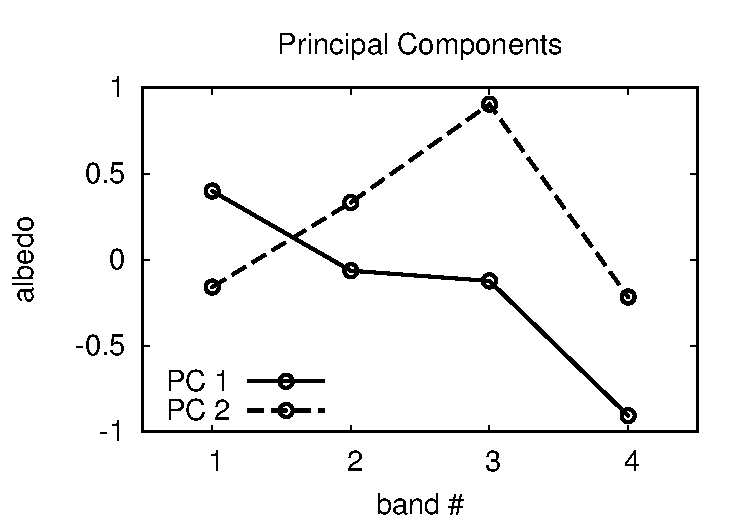
\includegraphics[width=0.9\hsize]{PCA_V_jn.pdf}
    \end{center}
    \caption{Principal Components. }
\label{fig:PCs}
\end{figure}
%%%%%%%%%%%%%%%%%%%%%%%%%%%%%%%%%%%


%%%%%%%%%%%%%%%%%%%%%%%%%%%%%%%%%%%
\begin{figure*}[b]
    \begin{center}
%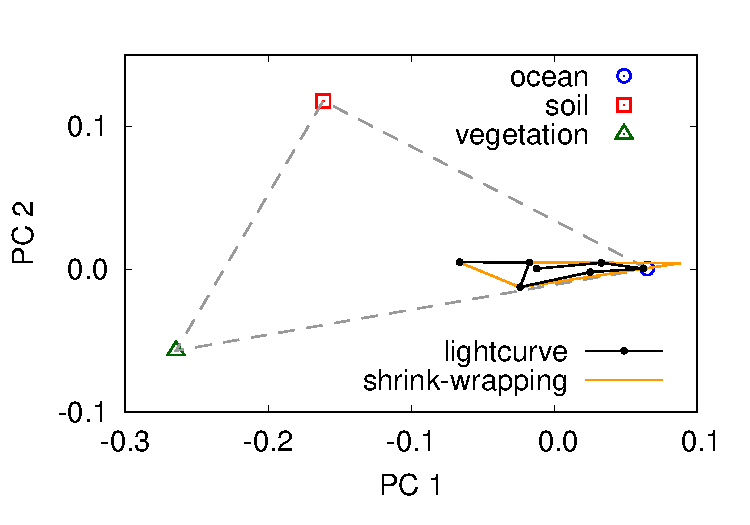
\includegraphics[width=\hsize]{PCA_projected.pdf}
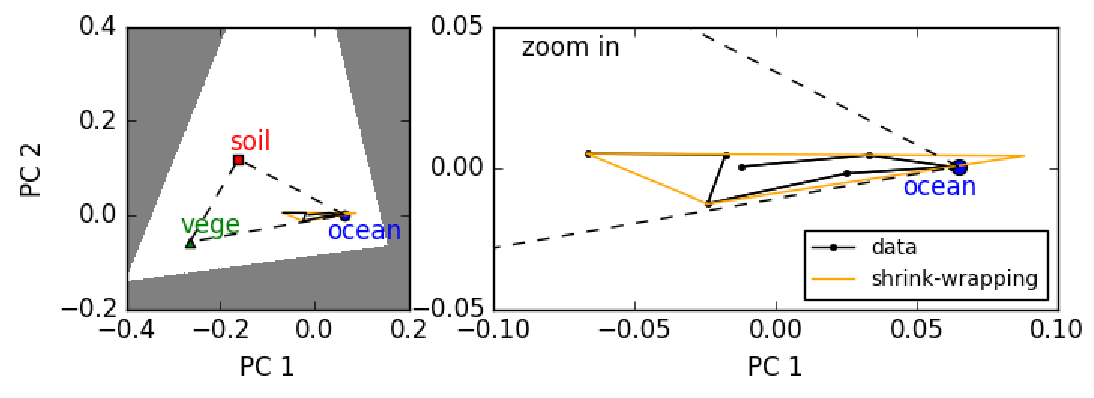
\includegraphics[width=\hsize]{mockdata_quadrature_PCplane.pdf}
    \end{center}
    \caption{Colors of 3 surface types and the light curves projected to the plane of 1st and 2nd principal components. }
\label{fig:shrinkwrap}
\end{figure*}
%%%%%%%%%%%%%%%%%%%%%%%%%%%%%%%%%%%

Then, we performed simplex shrink-wrapping analysis in the plane defined by these two principal components, based on the algorithm described in \citet{Fuhrmann1999}. 
The result are presented in Figure \ref{fig:shrinkwrap}. 
The black solid line indicates the trajectory of the light curves projected in this plane. 
The minimum-volume triangle that encloses the data points are found at the orange line in the same figure. 
For reference, the locations of the assumed three surface colors projected onto this plane are shown as points. 
As can be seen, the light curves the minimum-volume enclosure does not match the colors of physical surfaces, except for ocean. 
This is a natural consequence from the fact that the soil and vegetation are minor components and never dominate the surface in the illuminated and visible area, while the apparent covering fraction of ocean comes close to unity. 



%%%%%%%%%%%%%%%%%%%%%%%%%%%%%%%%%%%
\begin{figure*}[!htbp]
    \begin{center}
\includegraphics[width=\hsize]{xmed_std_regtime_l1e-2.pdf}
    \end{center}
    \caption{Result of estimation for $\{ \fast,\,s\}$ with $\lambda = 0.01$. \memoYF{MC chains do not fully converge in 5000 steps. The evolution of the chains are very weird.}}
    \label{fig:shrinkwrap}
\end{figure*}
%%%%%%%%%%%%%%%%%%%%%%%%%%%%%%%%%%%


%%%%%%%%%%%%%%%%%%%%%%%%%%%%%%%%%%%
\begin{figure*}[!htbp]
    \begin{center}
\includegraphics[width=\hsize]{xmed_std_regtime_l1e-4.pdf}
    \end{center}
    \caption{Result of estimation for $\{ \fast,\,s\}$ with $\lambda = 0.0001$. \memoYF{MC chains do not fully converge in 5000 steps.}}
\label{fig:shrinkwrap}
\end{figure*}
%%%%%%%%%%%%%%%%%%%%%%%%%%%%%%%%%%%


%%%%%%%%%%%%%%%%%%%%%%%%%%%%%%%%%%%
\begin{figure*}[!htbp]
    \begin{center}
\includegraphics[width=\hsize]{xmed_std_reglong_l1e-2.pdf}
    \end{center}
    \caption{Result of estimation for $\{ f,\,s\}$ with $\lambda = 0.01$. \memoYF{MC chains do not fully converge in 5000 steps, and it is not a single peak!!}}
\label{fig:xmed_std_reglong_l1e-2}
\end{figure*}
%%%%%%%%%%%%%%%%%%%%%%%%%%%%%%%%%%%


%%%%%%%%%%%%%%%%%%%%%%%%%%%%%%%%%%%
\begin{figure*}[!htbp]
    \begin{center}
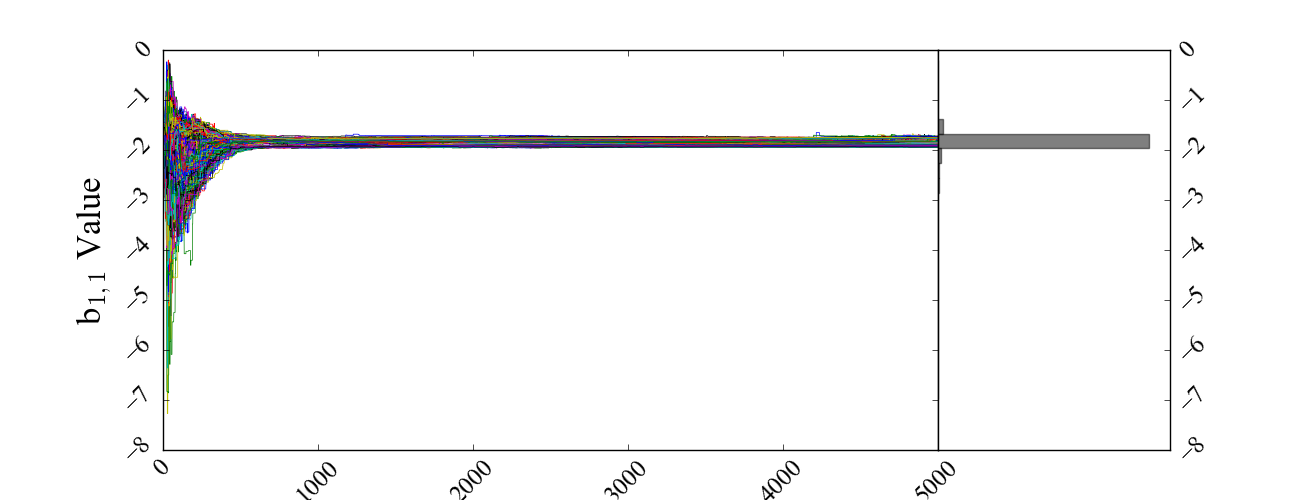
\includegraphics[width=\hsize]{reglong_l1e-2_trace0.png}
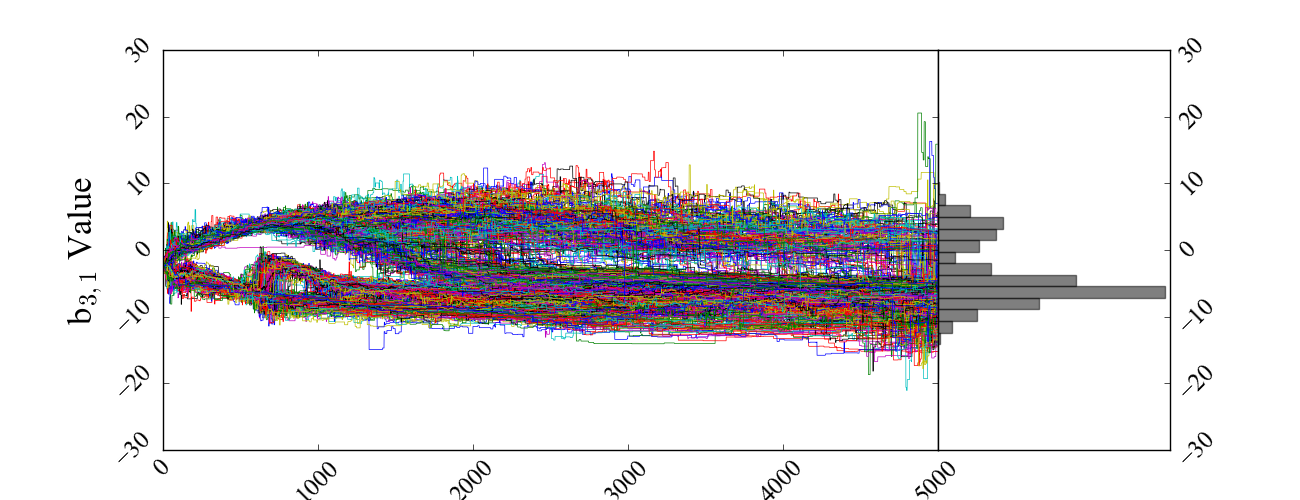
\includegraphics[width=\hsize]{reglong_l1e-2_trace8.png}
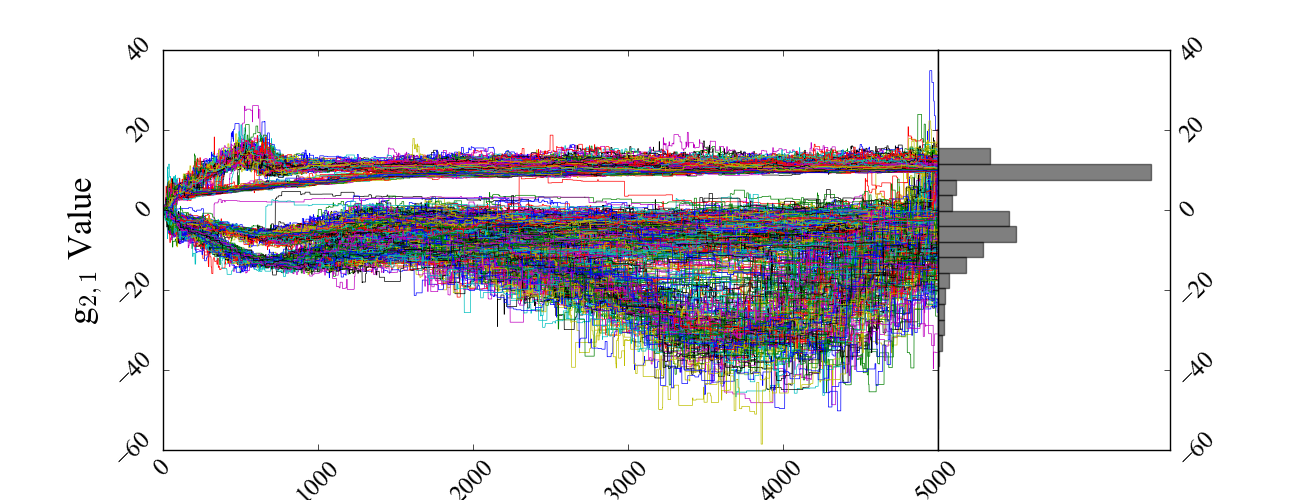
\includegraphics[width=\hsize]{reglong_l1e-2_trace13.png}
    \end{center}
    \caption{Examples of MC chains in estimating $\{ f,\,s\}$ with $\lambda = 0.01$, corresponding to Figure \ref{fig:xmed_std_reglong_l1e-2}. }
\label{fig:shrinkwrap}
\end{figure*}
%%%%%%%%%%%%%%%%%%%%%%%%%%%%%%%%%%%


%%%%%%%%%%%%%%%%%%%%%%%%%%%%%%%%%%%
%\begin{figure*}[!htbp]
%    \begin{center}
%\includegraphics[width=\hsize]{xmed_std_reglong_s1e-4.pdf}
%    \end{center}
%    \caption{Result of estimation for $\{ f,\,s\}$ with $\lambda = 0.0001$. \memoYF{MC chains do not fully converge in 5000 steps.}}
%\label{fig:shrinkwrap}
%\end{figure*}
%%%%%%%%%%%%%%%%%%%%%%%%%%%%%%%%%%%


%%%%%%%%%%%%%%%%%%%%%%%%%%%%%%%%%%%
%\begin{figure*}[!htbp]
%    \begin{center}
%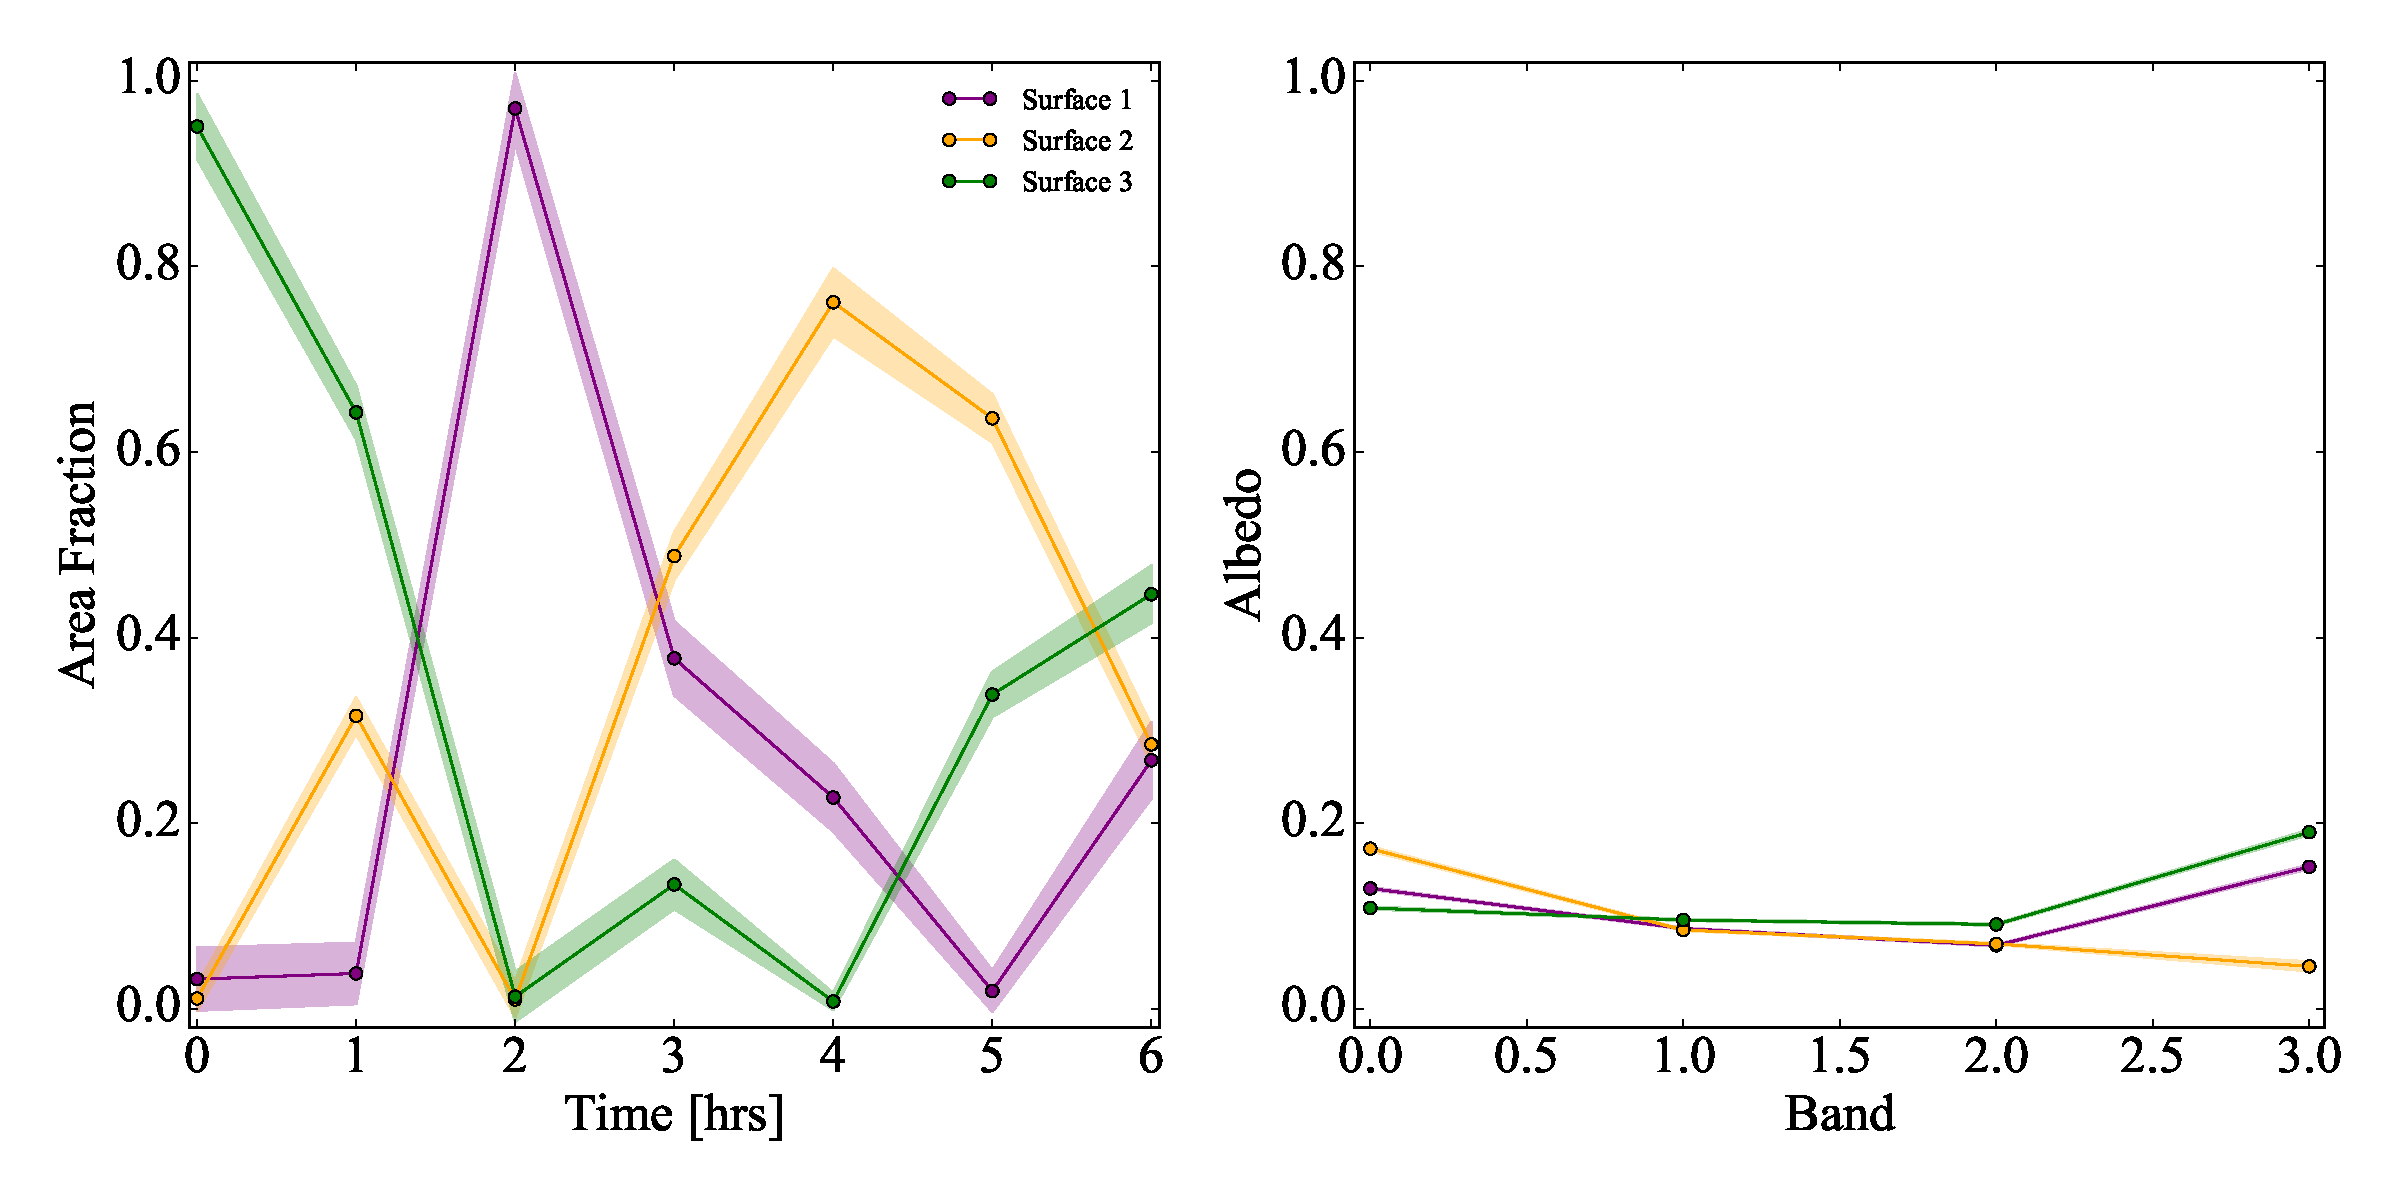
\includegraphics[width=\hsize]{xmed_std_time.pdf}
%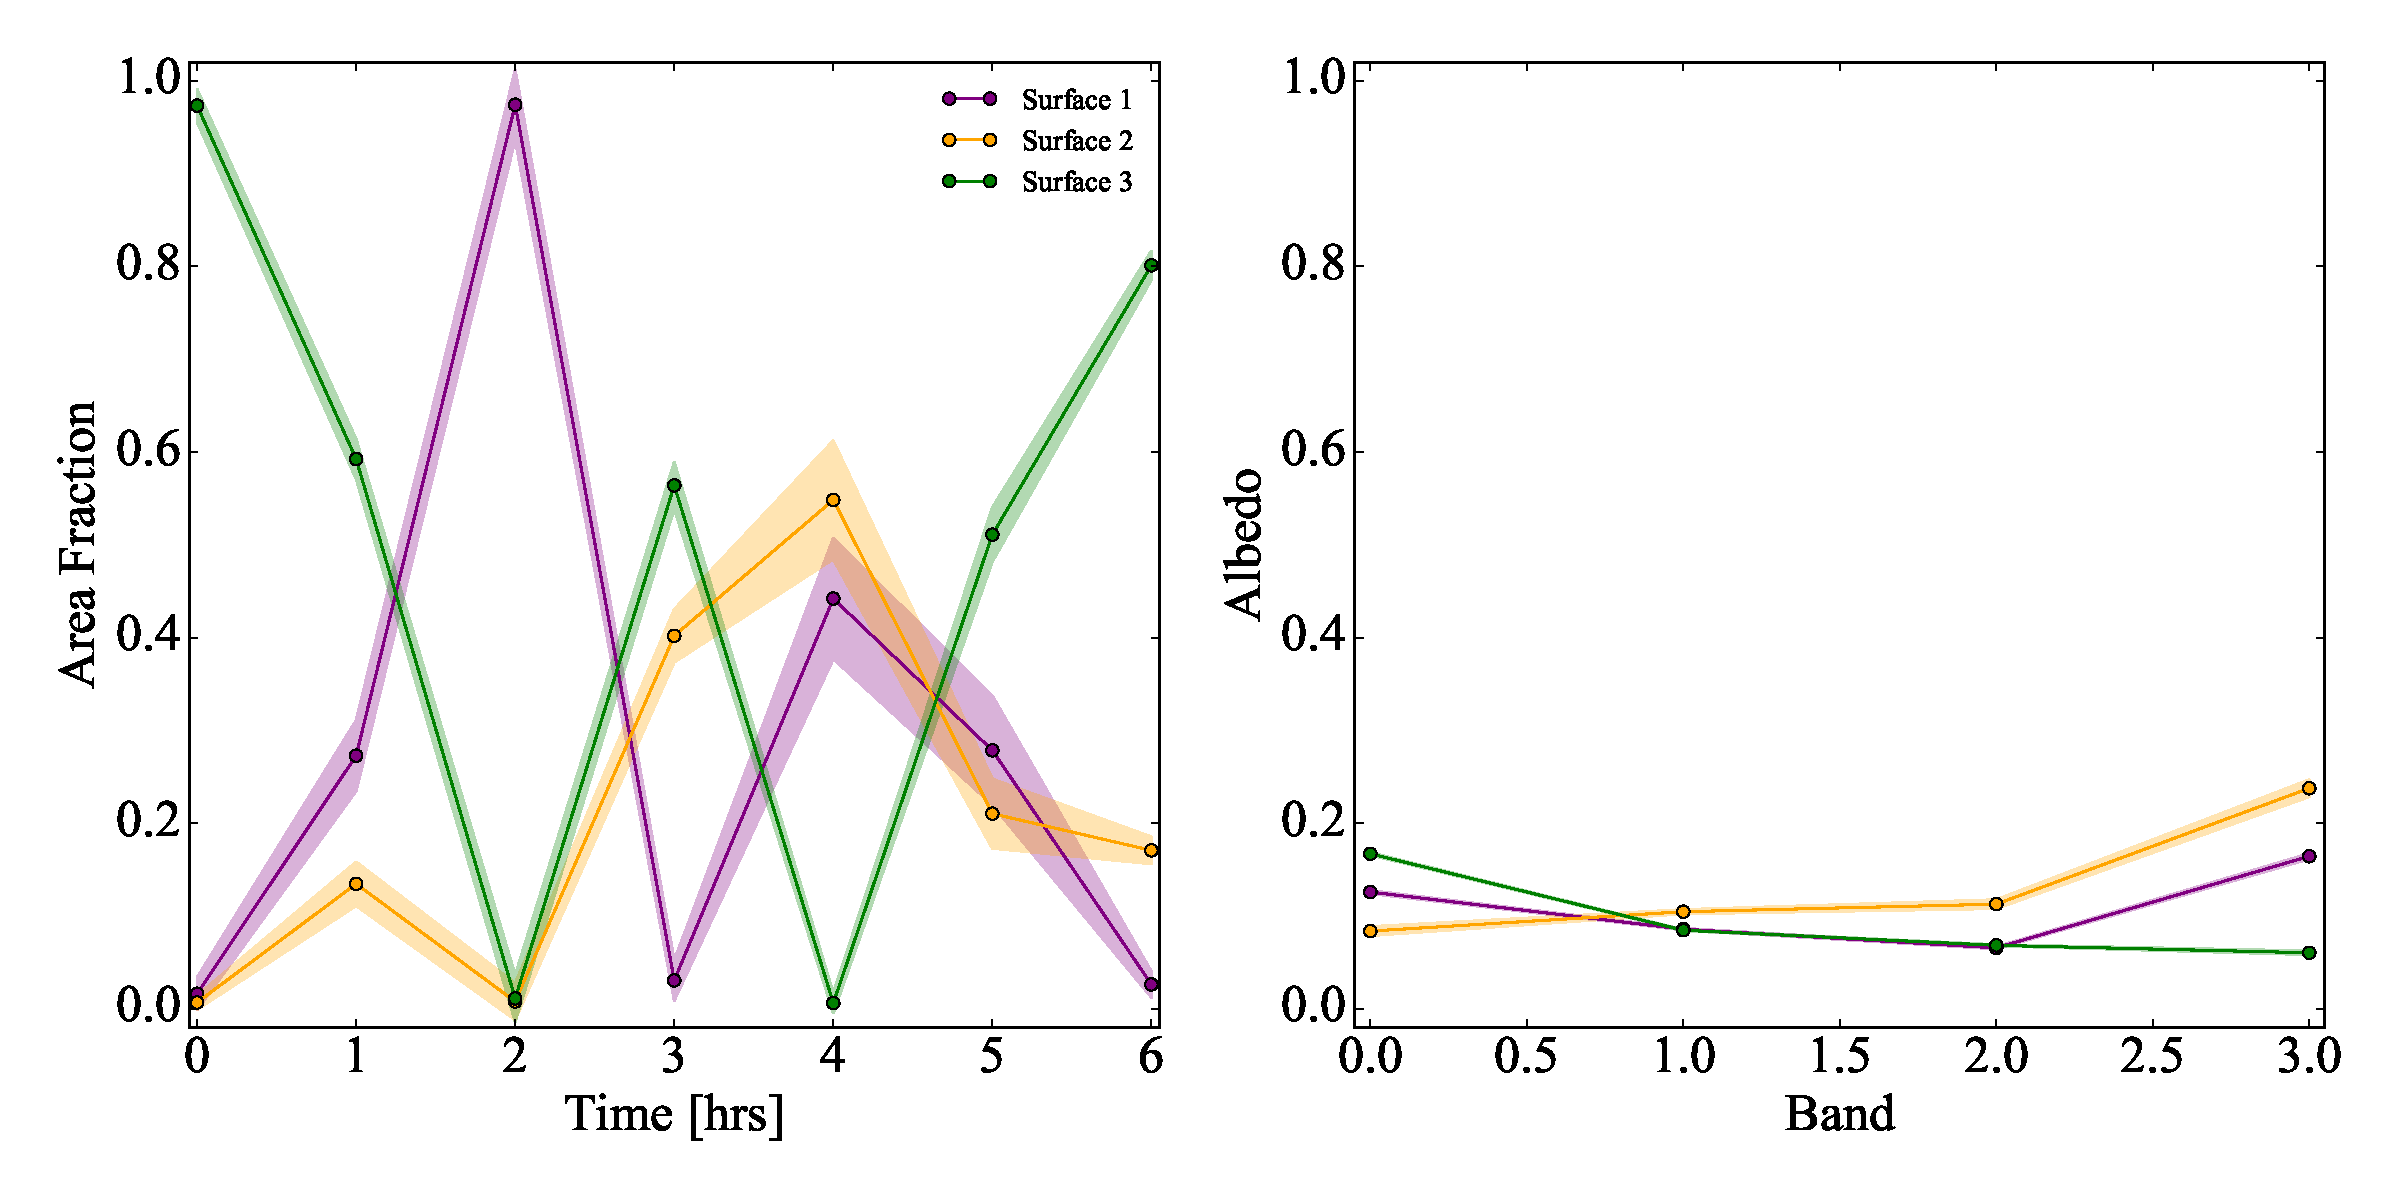
\includegraphics[width=\hsize]{xmed_std_longitude.pdf}
%    \end{center}
%    \caption{Left: result of estimation for $\{ \fast,\,s\}$. Right: result of estimation for $\{ f,\,s\}$}
%\label{fig:shrinkwrap}
%\end{figure*}
%%%%%%%%%%%%%%%%%%%%%%%%%%%%%%%%%%%




\clearpage

\acknowledgments

\bibliography{ref}

\newpage

\appendix

%%%%%%%%%%%%%%%%%%%%%%%%%%%%%%%%%%%%%%%%%%%%%%%%%%%%%%%%%%%%%%%%%%%
\section{Application to 4 EPOXI observations of the Earth}
\label{s:epoxi}
%%%%%%%%%%%%%%%%%%%%%%%%%%%%%%%%%%%%%%%%%%%%%%%%%%%%%%%%%%%%%%%%%%%

%%%%%%%%%%%%%%%%%%%%%%%%%%%%%%%%%%%%%%%%%%%%%%%%%%%%%%%%%%%%%%
\subsection{EPOXI data}
\label{ss:epoxidata}
%%%%%%%%%%%%%%%%%%%%%%%%%%%%%%%%%%%%%%%%%%%%%%%%%%%%%%%%%%%%%%

%%%%%%%%%%%%%%%%%%%%%%%%%%%%%%%%%%%
\begin{figure*}[b!]
    \begin{center}
\includegraphics[width=\hsize]{EPOXI_vislightcurve_4obs.pdf}
    \end{center}
    \caption{4 light curves of the Earth obtained with EPOXI mission.}
\label{fig:EPOXIlc}
\end{figure*}
%%%%%%%%%%%%%%%%%%%%%%%%%%%%%%%%%%%

We now apply our framework to the observed multi-band reflected light curves of the Earth obtained with EPOXI \citep{Livengood2011, Cowan2011}. 
There are 7 photometric filters from about 300 nm to 1000 nm, each of which has roughly 100-nm band width. 
In total, 5 series of observations were conducted, each of which spans $\sim $24 hours with 1-hour intervals. 
Since one of them includes lunar transit in front of the Earth and the interpretation is not straightforward, we just remove it from our data and consider only 4 series of observations, which were conducted on March 2008, June 2008, March 2009, and October 2009. 
The data are presented in Figure \ref{fig:EPOXIlc} in terms of {\it apparent albedo}. 

The geometrical configuration among the star, the target (the Earth), and the detector varies from observation to observation. 
The information is summarized in \citet{Cowan2011}, but we also outline in Table \ref{tab:EPOXI} just for reference. 

%%%%%%%%%%%%%%%%%%%%%%%%%%%%%%%%%%%
\begin{figure*}[!bt]
    \begin{center}
    \includegraphics[width=\hsize]{June_xmed_std_GPReg.pdf}
    \end{center}
    \caption{Result of inversion of EPOXI June data. \memoYF{to be revised}}
\label{fig:mcmc_June_tmp}
\end{figure*}
%%%%%%%%%%%%%%%%%%%%%%%%%%%%%%%%%%%

%%%%%%%%%%%%%%%%%%%%%%%%%%%%%%%%%%%
\begin{table*}[htp]
\caption{EPOXI Observations}
\begin{center}
\begin{tabular}{lcccc} \hline \hline
& Equator (equinox) & Equator (solstice) & North & South \\ \hline
Date & 2008 Mar 18-19 & 2008 Jun 4-5 & 2009 Mar 27-28 & 2009 Oct 4-5 \\ 
Phase & $57.7^{\circ }$ & $76.6^{\circ }$ & $85.9^{\circ }$ & $86.4^{\circ }$ \\ 
average sub-solar latitude & $-0.4^{\circ }$ & $22.6^{\circ }$ & $3.0^{\circ }$ & $-4.6^{\circ }$ \\
average sub-observer latitude & $1.6^{\circ }$ & $0.3^{\circ }$ & $61.5^{\circ }$ & $-73.7^{\circ }$  \\
initial sub-solar longitude & $267.6^{\circ }$ & $286.0^{\circ }$ & $296.7^{\circ }$ & $33.2^{\circ }$ \\
initial sub-observer longitude & $210.1^{\circ }$ & $210.5^{\circ }$ & $210.1^{\circ }$ & $300.6^{\circ }$ \\ \hline
\end{tabular}
\end{center}
\label{tab:EPOXI}
\end{table*}%
%%%%%%%%%%%%%%%%%%%%%%%%%%%%%%%%%%%


\end{document}
